\documentclass[a4paper,12pt,twoside]{article}
\usepackage[margin=0.9in]{geometry}

\usepackage[utf8]{inputenc}
\usepackage[pdftex]{graphicx}
\usepackage{polski}
\usepackage{amsfonts}
\usepackage{verbatim}
\usepackage{listings}
\usepackage{color}
\usepackage{enumitem}
\usepackage{tabularx}
\tolerance=1000
\setcounter{secnumdepth}{4}

% Bez kolorowania slow kluczowych
\lstset{language=, frame=single, breaklines=true, basicstyle=\footnotesize}

\newcommand{\parsection}[1]{\paragraph{#1}\mbox{}\\\\}

% wyroznienie slow kluczowych
\newcommand{\tech}{\texttt}

%wielowyrazowe nazwy ktore trzeba wyroznic
\newcommand{\name}{\textsl}

%%%%%%%%%%%%%%%%%%%%%%%%%%%%%%%%%%%%%%%%%%%%%%%%%%%%%%%%%%%%%%%%%%%%%%%%%%%%%%%%%%%%%%%%%%%%%%%%%%%%%%%%%%%%
\title{ Eksploracja Danych - Projekt}

\author{ Mateusz Supronowicz \\ Maciej Pietrzak}
%%%%%%%%%%%%%%%%%%%%%%%%%%%%%%%%%%%%%%%%%%%%%%%%%%%%%%%%%%%%%%%%%%%%%%%%%%%%%%%%%%%%%%%%%%%%%%%%%%%%%%%%%%%%

\begin{document}
\maketitle

%%%%%%%%%%%%%%%%%%%%%%%%%%%%%%%%%%%%%%%%%%%%%%%%%%%%%%%%%%%%%%%%%%%%%%%%%%%%%%%%%%%%%%%%%%%%%%%%%%%%%%%%%%%%
\section{Wprowadzenie}
\bigskip
%%%%%%%%%%%%%%%%%%%%%%%%%%%%%%%%%%%%%%%%%%%%%%%%%%%%%%%%%%%%%%%%%%%%%%%%%%%%%%%%%%%%%%%%%%%%%%%%%%%%%%%%%%%%


\subsection{Cel projektu}

Celem projektu jest przeprowadzenie analizy, grupowania i klasyfikacji na rzeczywistych danych.
Nasza grupa otrzymała próbki szkła (plik ``szklo\_B.mat'') z następującymi parametrami fizykochemicznymi:
\begin{enumerate}
\item Współczynnik załamania światła
\item Zawartość sodu (Na)
\item Zawartość magnezu (Mg)
\item Zawartość aluminium (Al)
\item Zawartość krzemu (Si)
\item Zawartość potasu (K)
\item Zawartość wapnia (Ca)
\item Zawartość baru (Ba)
\item Zawartość żelaza (Fe)
\end{enumerate}

W celu dogłębnej analizy danych wykorzystane zostaną metody poznane na wykładach, wdrożone za
pomocą języka ``R''.

\subsection{Środowisko, narzędzia}

System operacyjny: Windows 8.1\\
IDE: R 3.1.2, RStudio 0.98\\
Inne narzędzia: Emacs 24.4.1\\

\subsection{Postanowienia ogólne}

Początkowym etapem pracy jest poprawne wczytanie danych z pliku i wybranie najistotniejszych
o nich informacji.

\medskip
\begin{lstlisting}
  # Wczytanie danych z pliku
  file <- readMat("szklo_B.mat")

  # Wczytanie macierzy
  data.mx <- file$szklo.B

  # Liczba wierszy i kolumn - zmienne pomocniczne
  data.row <- nrow(data.mx)
  data.col <- ncol(data.mx)
\end{lstlisting}
\medskip

Dla lepszych obserwacji szeregowo ugrupowanych danych - są one często przedstawione
poniżej w postaci macierzy kolumnowej zamiast wektora.\\

Atrybutom przedstawionym w celach projektu przypisana jest numeracja, za pomocą której
będą owe atrybuty będą w tym dokumencie przedstawiane.

%%%%%%%%%%%%%%%%%%%%%%%%%%%%%%%%%%%%%%%%%%%%%%%%%%%%%%%%%%%%%%%%
\section{Zadanie 1}
\bigskip
%%%%%%%%%%%%%%%%%%%%%%%%%%%%%%%%%%%%%%%%%%%%%%%%%%%%%%%%%%%%%%%%

Pierwszym zadaniem było określenie następujących  parametrów dotyczących danych t.j.:

\begin{itemize}
\item Liczba próbek i atrybutów
\item Wartości średnie poszczególnych atrybutów
\item Odchylenia standardowe
\item Zakresy zmienności atrybutów
\end{itemize}

Warto spojrzeć na podstawowe parametry danych by lepiej się z nimi zapoznać:

\medskip
\begin{lstlisting}
  > summary(data.mx)

       V1              V2              V3              V4
  Min.   :1.511   Min.   :11.02   Min.   :0.000   Min.   :0.290
  1st Qu.:1.516   1st Qu.:12.92   1st Qu.:1.845   1st Qu.:1.188
  Median :1.518   Median :13.32   Median :3.480   Median :1.360
  Mean   :1.518   Mean   :13.43   Mean   :2.650   Mean   :1.438
  3rd Qu.:1.519   3rd Qu.:13.87   3rd Qu.:3.600   3rd Qu.:1.570
  Max.   :1.534   Max.   :17.38   Max.   :4.490   Max.   :3.500

       V5              V6               V7
  Min.   :69.89   Min.   :0.0000   Min.   : 5.430
  1st Qu.:72.34   1st Qu.:0.1200   1st Qu.: 8.240
  Median :72.78   Median :0.5500   Median : 8.630
  Mean   :72.69   Mean   :0.5096   Mean   : 8.952
  3rd Qu.:73.10   3rd Qu.:0.6000   3rd Qu.: 9.140
  Max.   :75.41   Max.   :6.2100   Max.   :16.190

       V8               V9
  Min.   :0.0000   Min.   :0.00000
  1st Qu.:0.0000   1st Qu.:0.00000
  Median :0.0000   Median :0.00000
  Mean   :0.1545   Mean   :0.05219
  3rd Qu.:0.0000   3rd Qu.:0.09000
  Max.   :2.8800   Max.   :0.37000
\end{lstlisting}
\medskip

Jak widać istnieje tu przewaga danych o wartościah \texttt{[0, 2]} z wyjątkiem \texttt{atrybutu nr.5},
którego wartości znajdują się w przedziale \texttt{[69.89, 75.41]} oraz \texttt{atrybutów nr.2 [11.02, 17.38]}
i \texttt{nr.7 [5.43, 16.19]}.

\subsection{Liczba próbek i atrybutów}

\begin{lstlisting}
  # Probki
  > data.row
  [1] 160

  # Atrybuty
  > data.col
  [1] 9
\end{lstlisting}

\subsection{Średnia}

Mimo, że do dalszych obliczeń potrzebna będzie tylko średnia arytmetyczna, pozwoliłem sobie także
obliczyć średnią harmoniczną i geometryczną.

\medskip
\begin{lstlisting}
  # Obliczanie srednich - arytmetyczna[,1], harmoniczna[,2], geometryczna[,3]
  mean.mx <- matrix( , nrow = data.col, ncol = 3)

  for(i in 1 : data.col) {
    mean.mx[i, ] <- c(mean(data.mx[ ,i]), harmonic.mean(data.mx[ ,i]), geometric.mean(data.mx[ ,i]))
  }

  # Otrzymane wartosci
  > mean.mx
             [,1]      [,2]      [,3]
  [1,]  1.5182619  1.518256  1.518259
  [2,] 13.4266250 13.377462 13.401880
  [3,]  2.6504375  0.000000  0.000000
  [4,]  1.4380625  1.245120  1.347667
  [5,] 72.6858125 72.677520 72.681675
  [6,]  0.5096250  0.000000  0.000000
  [7,]  8.9516875  8.766439  8.853824
  [8,]  0.1545000  0.000000  0.000000
  [9,]  0.0521875  0.000000  0.000000
\end{lstlisting}

\begin{center}
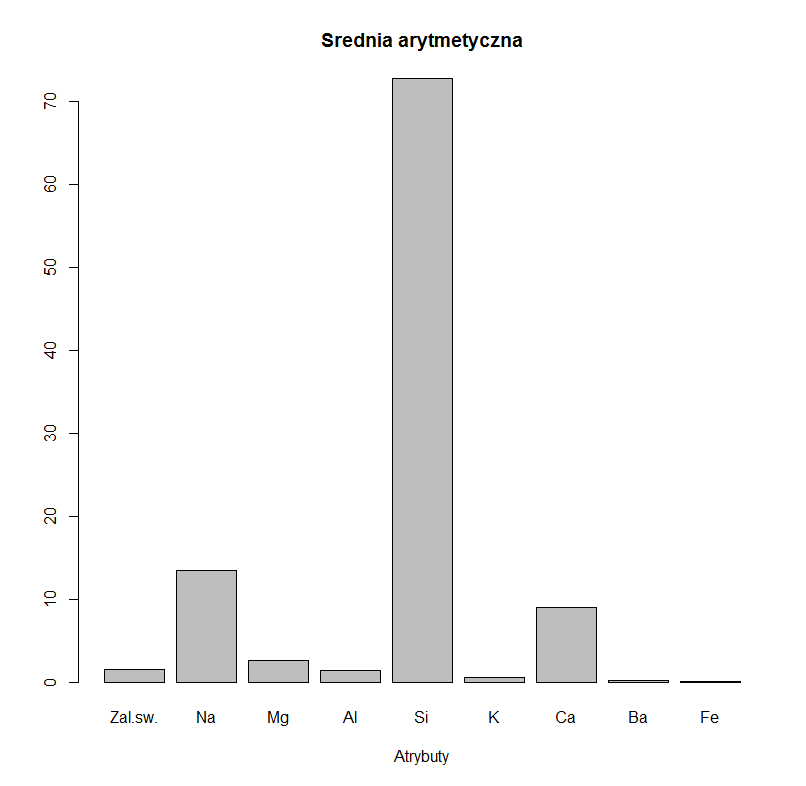
\includegraphics[width=.9\textwidth]{img/1_srednia_arytmetyczna.png}
\end{center}

\subsection{Odchylenie standardowe}

\begin{lstlisting}
  # Odchylenie standardowe atrybutow

  stddev.mx <- matrix( ,nrow = data.col, ncol = 1)
  for(i in 1 : data.col) {
    stddev.mx[i, ] = sd(data.mx[ ,i])
  }

  > stddev.mx
              [,1]
  [1,] 0.002979884
  [2,] 0.825376520
  [3,] 1.461072815
  [4,] 0.516487285
  [5,] 0.776487391
  [6,] 0.733870490
  [7,] 1.430254946
  [8,] 0.446910850
  [9,] 0.091930189
\end{lstlisting}

\begin{center}
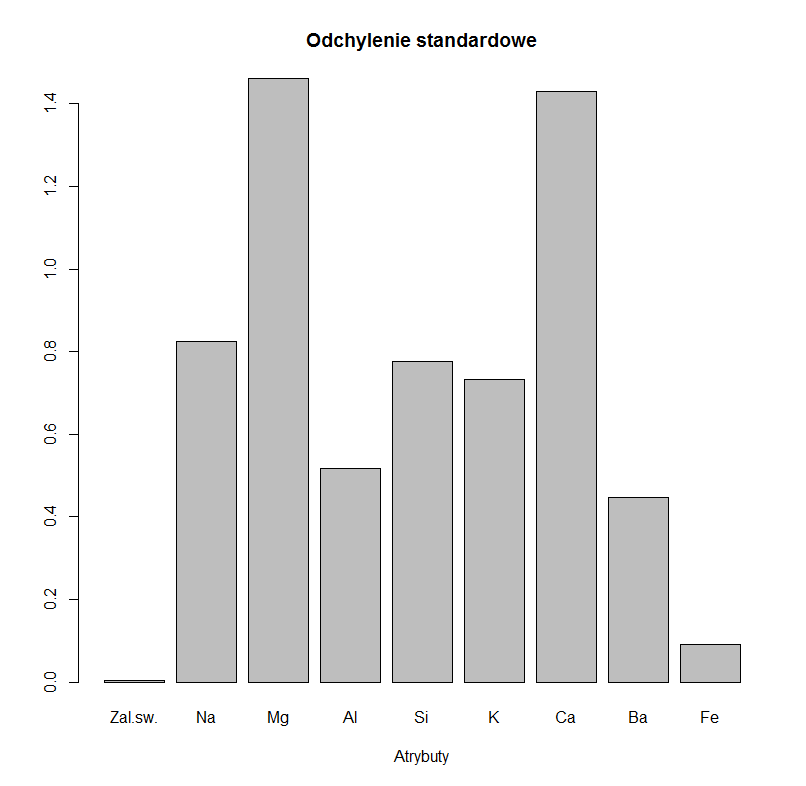
\includegraphics[width=.9\textwidth]{img/1_odchylenie_standardowe.png}
\end{center}

\subsection{Rozstęp wartości poszczególnych atrybutów}

\begin{lstlisting}
  range.mx <- matrix( , nrow = data.col, ncol = 2) # Wartosci min, max
  diff.mx <- matrix( , nrow = data.col, ncol = 1)  # Rozstep

  for(i in 1 : data.col) {
    range.mx[i, ] <- range(data.mx[ ,i])
    diff.mx[i, ] <- diff(range.mx[i, ])
  }

  # Wartosci min[,1] i max[,2] poszczegolnych atrybutow
  > range.mx
           [,1]     [,2]
  [1,]  1.51115  1.53393
  [2,] 11.02000 17.38000
  [3,]  0.00000  4.49000
  [4,]  0.29000  3.50000
  [5,] 69.89000 75.41000
  [6,]  0.00000  6.21000
  [7,]  5.43000 16.19000
  [8,]  0.00000  2.88000
  [9,]  0.00000  0.37000

  # Rozstep dla poszczegolnych atrybutow
  > diff.mx
           [,1]
  [1,]  0.02278
  [2,]  6.36000
  [3,]  4.49000
  [4,]  3.21000
  [5,]  5.52000
  [6,]  6.21000
  [7,] 10.76000
  [8,]  2.88000
  [9,]  0.37000
\end{lstlisting}

\begin{center}
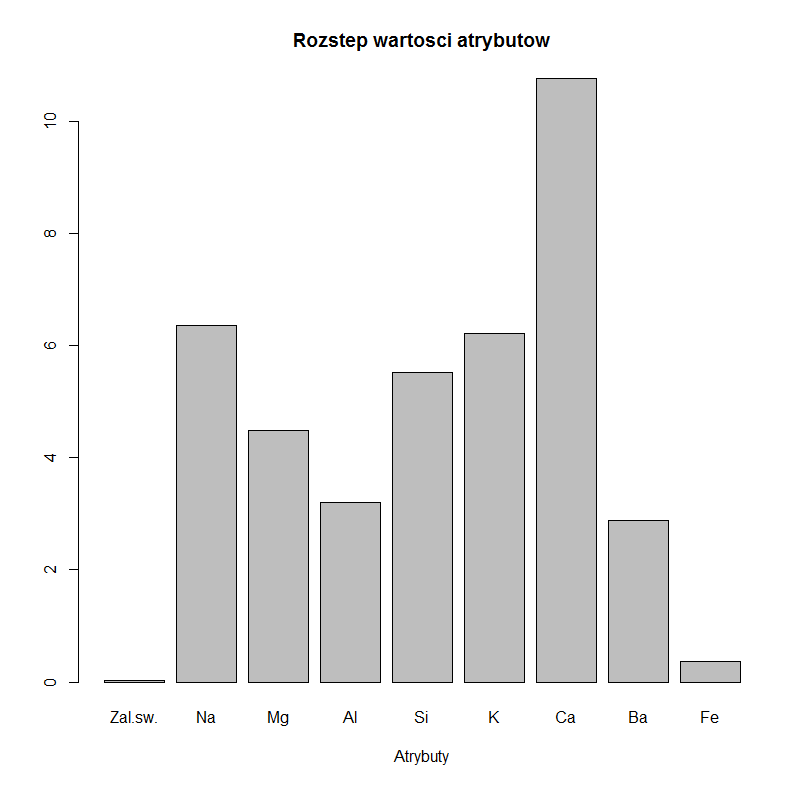
\includegraphics[width=.90\textwidth]{img/1_rozstep_wartosci.png}
\end{center}

\subsection{Miara zmienności poszczególnych atrybutów}

\begin{lstlisting}
  # Miara zmiennosci poszczegolnych atrybutow
  cov.mx <- matrix( , nrow = data.col, ncol = 1)

  for(i in 1 : data.col) {
    cov.mx[i, ] <- stddev.mx[i, ] / mean.mx[i,1]
  }

  > cov.mx
              [,1]
  [1,] 0.001962694
  [2,] 0.061473119
  [3,] 0.551257222
  [4,] 0.359154964
  [5,] 0.010682792
  [6,] 1.440020584
  [7,] 0.159774897
  [8,] 2.892626863
  [9,] 1.761536550
\end{lstlisting}

\begin{center}
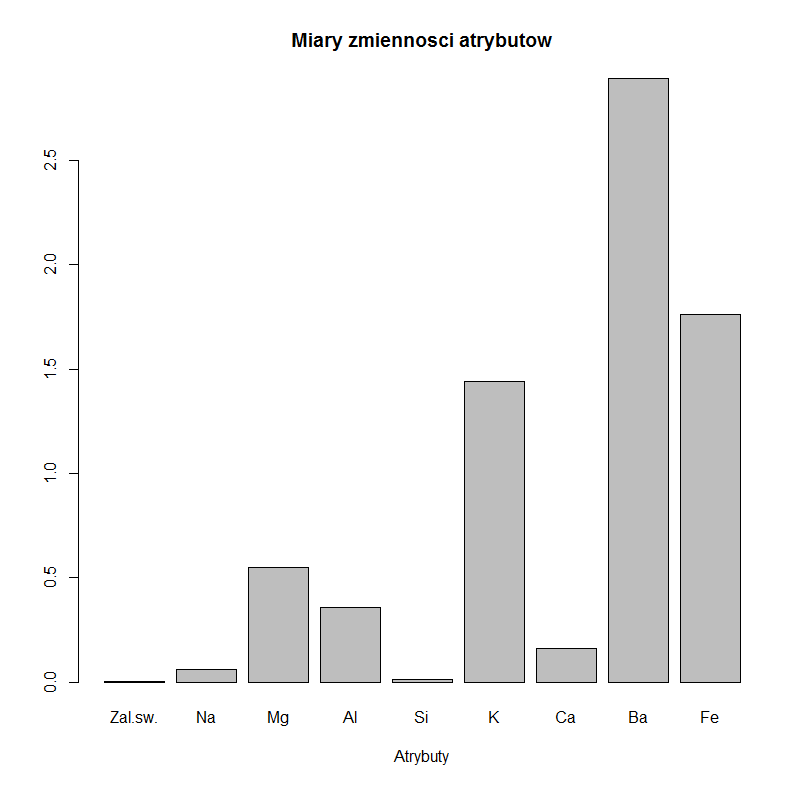
\includegraphics[width=.90\textwidth]{img/1_miary_zmiennosci.png}
\end{center}

\subsection{Analiza danych}

Zgodnie z miarami rozstępu i odchylenia standardowego najmniejszą zmienność wykazuje \texttt{atrybut nr.1}
(Załamanie światła) - \texttt{stddev[1,1] =  0.002979884, diff.mx[1,1] = 0.02278]}. Przemawia także za tym
pomocnicza miara zmienności \texttt{cov.mx[1,1] = 0.001962694}.\\

Największą zmiennością jednakże wykazuje się \texttt{atrybut nr.7 - stddev.mx[7,1] = 1.430254946,}
\texttt{diff.mx[7,1] = 10.76000}.
Co ciekawe obliczona miara zmienności pokazuje zupełnie co innego - największą zmienność wykazuje
\texttt{atrybut nr.8}. Przyglądając się jednak bliżej wartościom, stwierdzamy, że główną przyczyną oceny są
punkty oddalone, które znacząco wpływają na nasz wynik. Tym właśnie punktom poświęcimy więcej czasu w zadaniu 2.

%%%%%%%%%%%%%%%%%%%%%%%%%%%%%%%%%%%%%%%%%%%%%%%%%%%%%%%%%%%%%%%%
\section{Zadanie 2}
\bigskip
%%%%%%%%%%%%%%%%%%%%%%%%%%%%%%%%%%%%%%%%%%%%%%%%%%%%%%%%%%%%%%%%

Zadanie drugie to znalezienie punktów oddalonych w poszczególnych atrybutach. Jak określiliśmy w podsumowaniu
zadania 1, w niektórych przypadkach znacząco zakłócają one oczekiwany wynik (\texttt{Atrybut nr.6,8,9}).\\

\subsection{Obliczenia}

Obliczmy zatem punkty oddalone i przedstawmy je graficznie. Za punkty oddalone uznajemy te, których odległość
od średniej arytmetycznej jest większa niż dwukrotność odchylenia standardowego.

\medskip
\begin{lstlisting}
  # Macierz klasyfikujaca obiekty oddalone
  pts.odd.mx <- matrix( , nrow = data.row, ncol = data.col)

  for(i in 1 : data.col) {
    # Wzor klasyfikujacy
    pts.odd.mx[ ,i] <- abs(data.mx[ ,i] - mean.mx[i,1]) < (2 * stddev.mx[i,1])

    plot(seq(1, data.row, by = 1),
         data.mx[ ,i],
         pch = 16,
         xlab = "Probki",
         ylab = "Wartosci",
         col = pts.odd.mx[ ,i] + 1,
          main = paste("Atrybut Nr.", toString(i)))
  }
\end{lstlisting}

\subsection{Wykresy}

Na wykresach czarne punkty odpowiadają punktom oddalonym. Numeracja atrybutów jest identyczna z tą,
przedstawioną w celach projektu.\\

\begin{center}
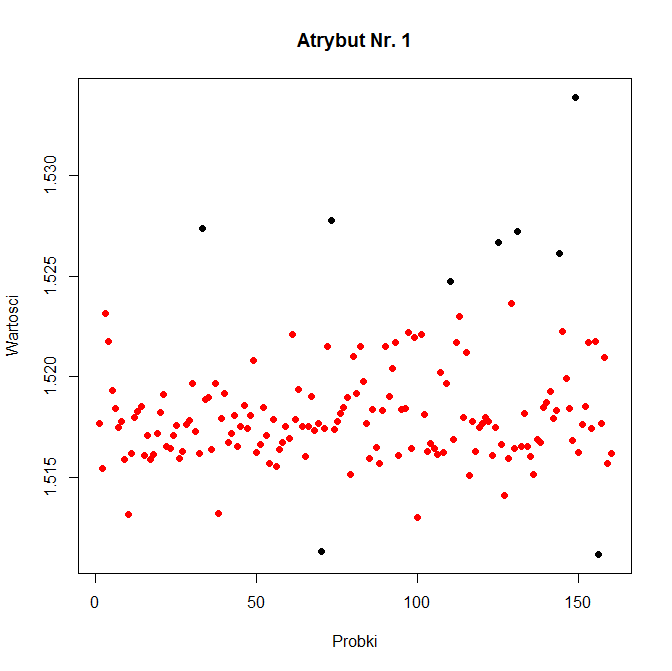
\includegraphics[width=.90\textwidth]{img/2_pkt_oddalone_1.png}
\end{center}

\begin{center}
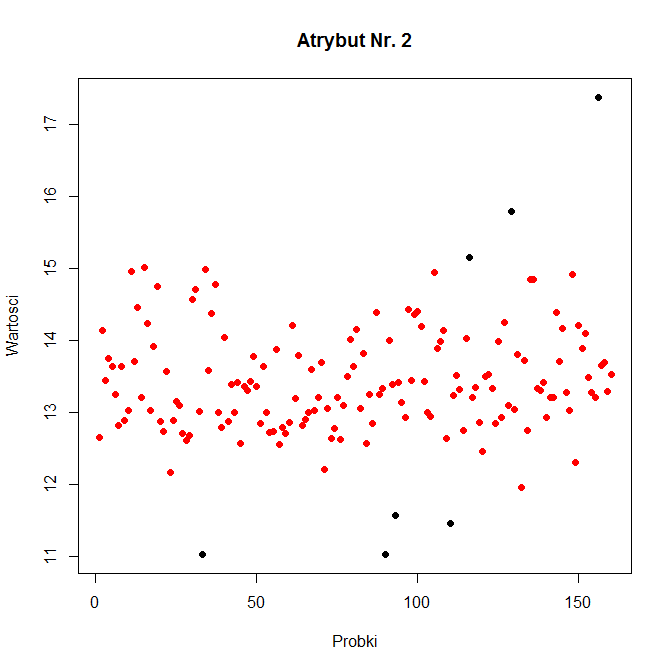
\includegraphics[width=.90\textwidth]{img/2_pkt_oddalone_2.png}
\end{center}

\begin{center}
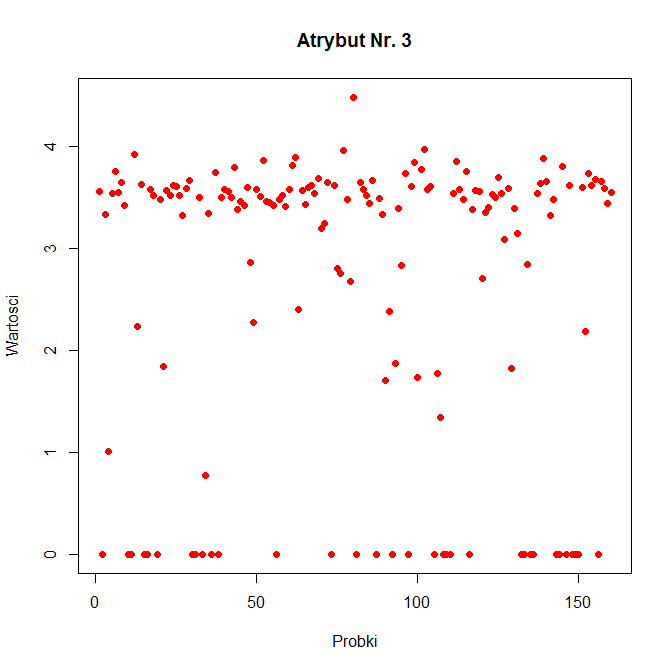
\includegraphics[width=.90\textwidth]{img/2_pkt_oddalone_3.png}
\end{center}

\begin{center}
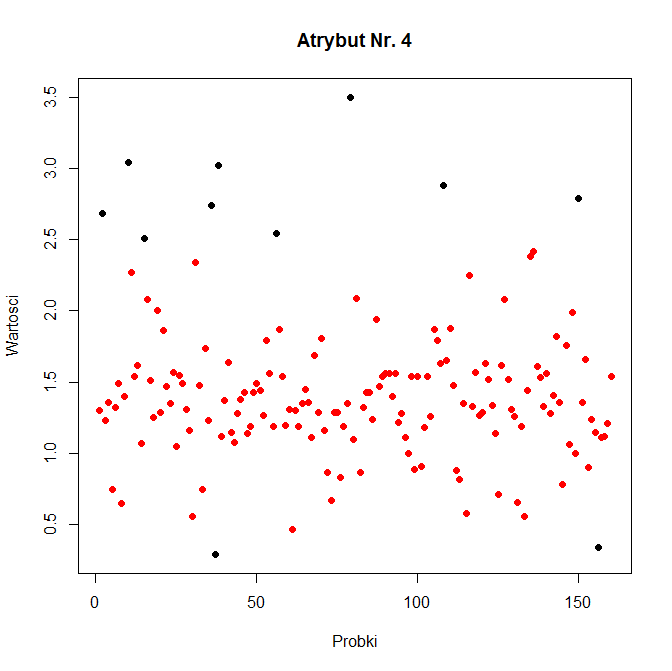
\includegraphics[width=.90\textwidth]{img/2_pkt_oddalone_4.png}
\end{center}

\begin{center}
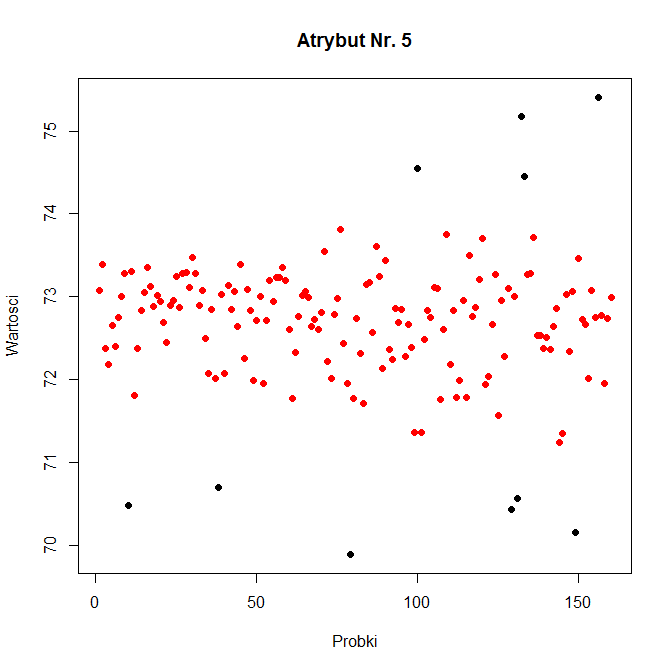
\includegraphics[width=.90\textwidth]{img/2_pkt_oddalone_5.png}
\end{center}

\begin{center}
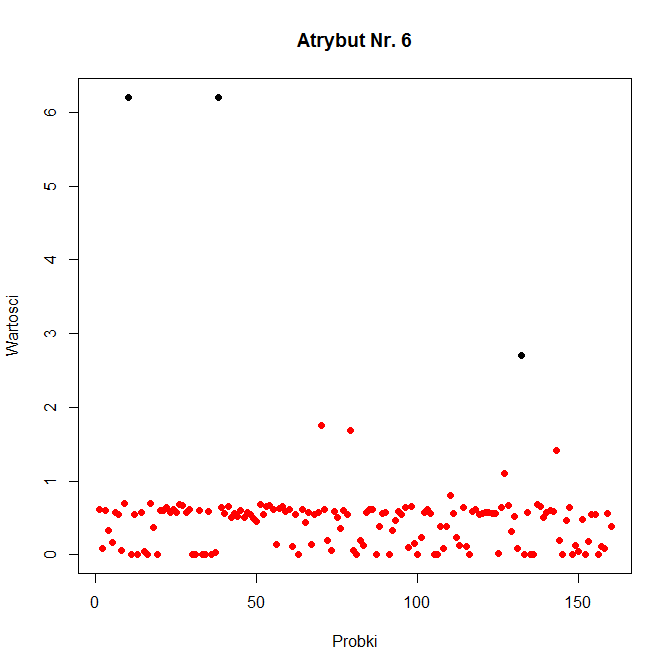
\includegraphics[width=.90\textwidth]{img/2_pkt_oddalone_6.png}
\end{center}

\begin{center}
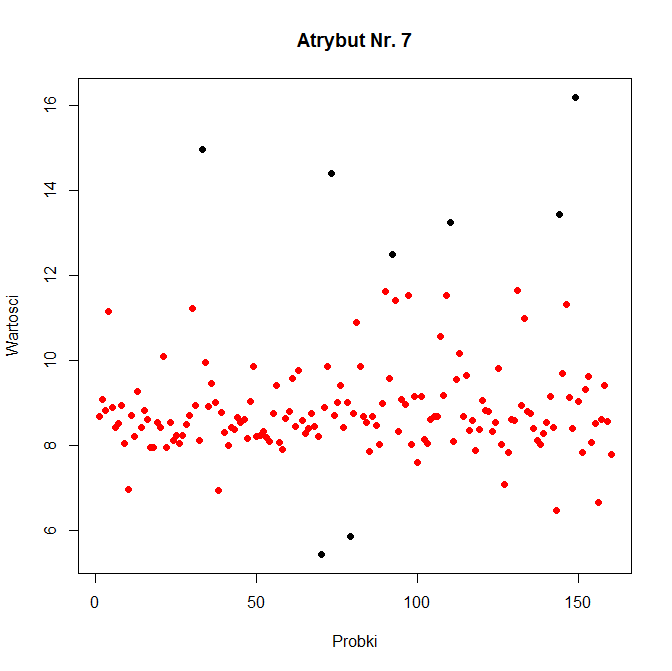
\includegraphics[width=.90\textwidth]{img/2_pkt_oddalone_7.png}
\end{center}

\begin{center}
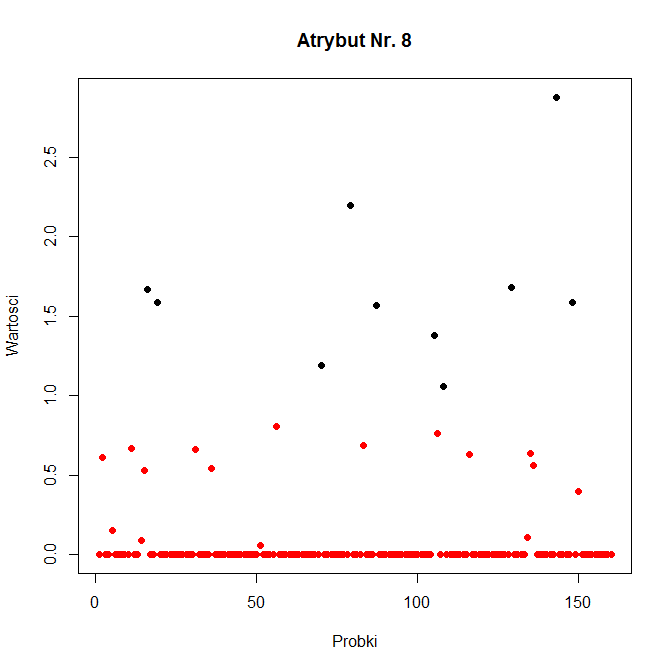
\includegraphics[width=.90\textwidth]{img/2_pkt_oddalone_8.png}
\end{center}

\begin{center}
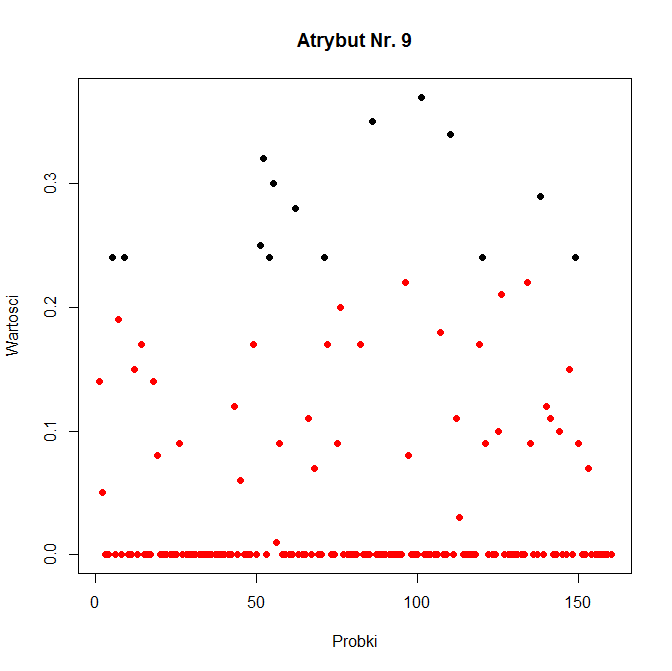
\includegraphics[width=.90\textwidth]{img/2_pkt_oddalone_9.png}
\end{center}

\subsection{Analiza}

Wykresy potwierdzają założenia, że punkty oddalone mogą znacznie zakłócić wynik.
Wszystkie atrybuty, oprócz nr.3, posiadają owe punkty.
Przyczynia się do tego nie tylko ich duża ilość np. jak w przypadku \texttt{atrybutu nr.9}
(gdybyśmy uznali za punkty oddalone większe niż jednokrotność odchylenia standardowego,
ich ilość byłaby znacznie większa), ale także ich duża odległość od średniej arytmetycznej - \texttt{atrybuty nr.2},
\texttt{nr.6} (Nawet wartość powyżej \texttt{6.0} przy średniej \texttt{0.5096250}), \texttt{nr.8, nr.9}.

Co ciekawe \texttt{atrybut nr.3} nie posiada punktów odległych. Jest zatem idealnym kandydatem, na którym
można efektywnie stosować metody eksploracyjne.

%%%%%%%%%%%%%%%%%%%%%%%%%%%%%%%%%%%%%%%%%%%%%%%%%%%%%%%%%%%%%%%%
\section{Zadanie 3}
\bigskip
%%%%%%%%%%%%%%%%%%%%%%%%%%%%%%%%%%%%%%%%%%%%%%%%%%%%%%%%%%%%%%%%

Kolejny etap naszej pracy to próba podzielenia próbek na grupy.

\subsection{Wartości}

Na początek umieściliśmy wartości wszystkich naszych atrybutów na jednym wykresie.

\medskip
\begin{lstlisting}
  # Pokazanie wszystkich danych na wykresie
  plot(data.mx[ ,1],
       pch = 16,
       col = 1,
       xlim = c(0, data.row), # Liczba probek
       ylim = c(min(data.mx), max(data.mx)),  # [min,max]
       xlab = "Indeks",
       ylab = "Wartosc",
       main = "Wartosci wszystkich atrybutow")

  for(i in 2 : data.col) {
    points(data.mx[ ,i], pch = 16, col = i)
  }
\end{lstlisting}

\begin{center}
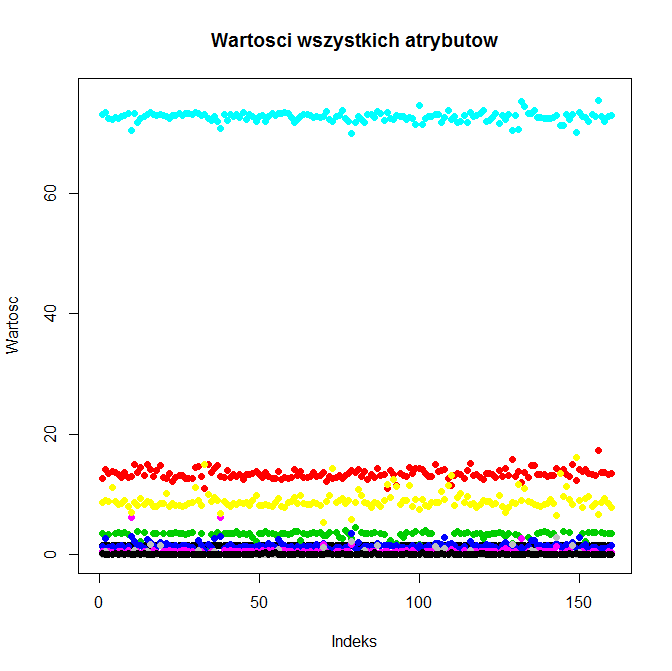
\includegraphics[width=.90\textwidth]{img/3_wszystkie_dane.png}
\end{center}

Po przeanalizowaniu wykresu można stwierdzić że ze względu na przyjmowane wartości dane te dzielą się
na 3 kategorie:

\begin{enumerate}
\item Dane, które przyjmują wartości najnizsze \texttt{\~[0, 8]} - \texttt{Atrybuty nr: 1,3,4,6,8,9}
\item Dane o wartościach nieco wyższych \texttt{\~[8, 10]} - \texttt{Atrybuty nr: 2,7}
\item Dane, o wartościach najwyższych \texttt{\~[70, 76]} - \texttt{Atrybut nr.5}
\end{enumerate}

\subsection{Punkty oddalone}

Warto także poddać analizie pełniącym dużą rolę punktom oddalonym. Badane zostaną \texttt{atrybuty nr.1,4,6,8,9}.

\medskip
\begin{lstlisting}
  # Rozpoznanie przedzialow w ktorych wystepuja punkty oddalone
  # w atrybutach nr. 1,4,6,8,9
  plot(data.mx[ ,1],
       pch = 16,
       col = pts.odd.mx[ ,1] + 1,
       xlim = c(0, data.row),
       ylim = c(0, 2),
       xlab = "Indeks",
       ylab = "Wartosci",
       main = "Wartosci punktow oddalonych przyjmowane w Atrybutach Nr. 1,4,6,8,9")

  points(data.mx[ ,9], pch = 16, col = pts.odd.mx[ ,9] + 1,
         xlim = c(0, data.row), ylim = c(0, 2))
  points(data.mx[ ,8], pch = 16, col = pts.odd.mx[ ,8] + 1,
         xlim = c(0, data.row), ylim = c(0, 2))
  points(data.mx[ ,6], pch = 16, col = pts.odd.mx[ ,6] + 1,
         xlim = c(0, data.row), ylim = c(0, 2))
  points(data.mx[ ,4], pch = 16, col = pts.odd.mx[ ,4] + 1,
         xlim = c(0, data.row), ylim = c(0, 2))

  axis(2, at = c(0.0, 0.2, 0.3, 0.4, 0.5, 1.0,
       1.2, 1.3, 1.4, 1.5, 1.6, 1.7, 2.0))
\end{lstlisting}

\begin{center}
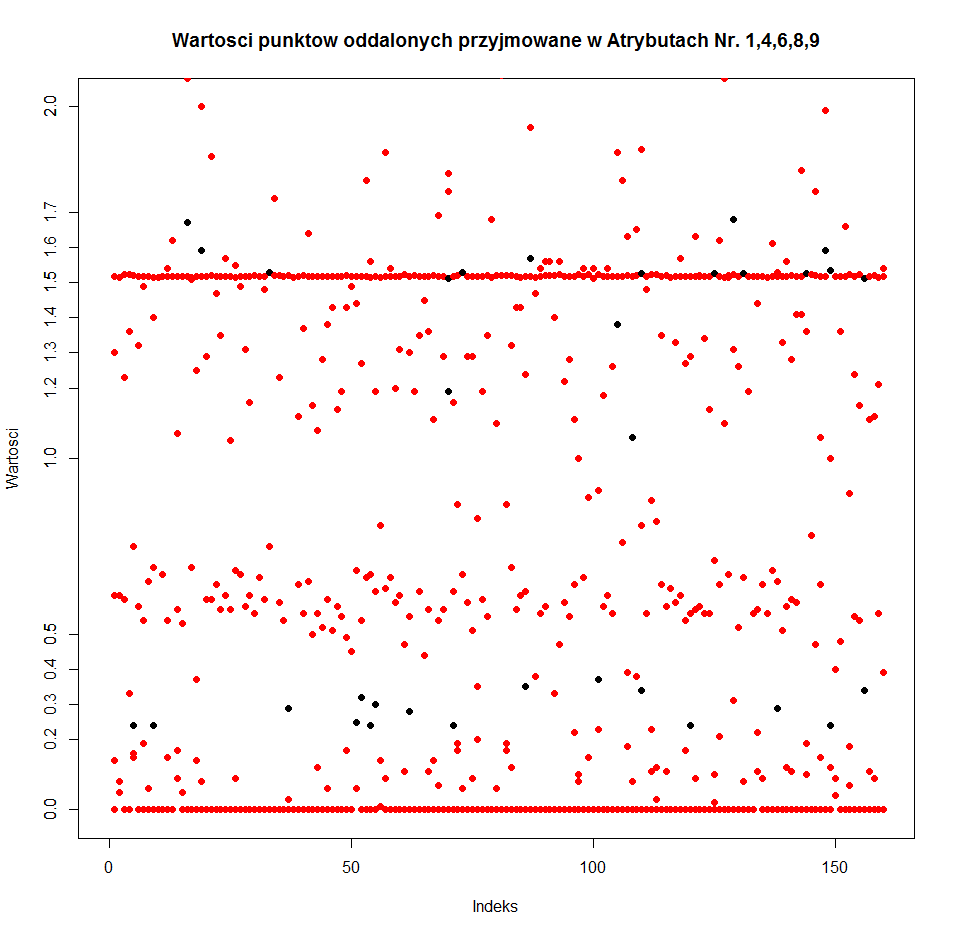
\includegraphics[width=.90\textwidth]{img/3_pkt_oddalone_14689.png}
\end{center}

Na przedstawionym wyżej wykresie czarnym kolorem zostały oznaczone punkty oddalone. Można zauważyć
pewien schemat. Otóż wartosci te ulokowane są:

\begin{itemize}
\item W przedziale \texttt{[0.2, 0.4]} - stanowiąc pierwszą wyłaniającą się grupę punktów oddalonych.
\item W przedziale \texttt{[1.4, 1.7]} - grupę drugą.
\end{itemize}

2 punkty w środkowej części wykresu wykluczamy z procesu grupowania.

\subsection{Macierz wykresów punktowych}

Przy procesie grupowania istotnym narzędziem jest macierz wykresów punktowych. Umieścilismy na niej
średnią, odchylenie standardowe, rozstęp danych i miarę zmienności dla poszczególnych atrybutów.

\medskip
\begin{lstlisting}
  # Macierz wykresow punktowych
  pairs(~mean.mx[ ,1] + stddev.mx + diff.mx + cov.mx,
        pch = 22,
        bg = rainbow(9),
	      oma = c(4,4,6,12),
	      main = "Macierz wykresow punktowych")

  par(xpd = TRUE)

  # Numery atrybutow i odpowiadajace im kolory
  legend(0.9, 0.7, c("1","2","3","4","5","6","7","8","9"), fill = rainbow(9))
\end{lstlisting}

\begin{center}
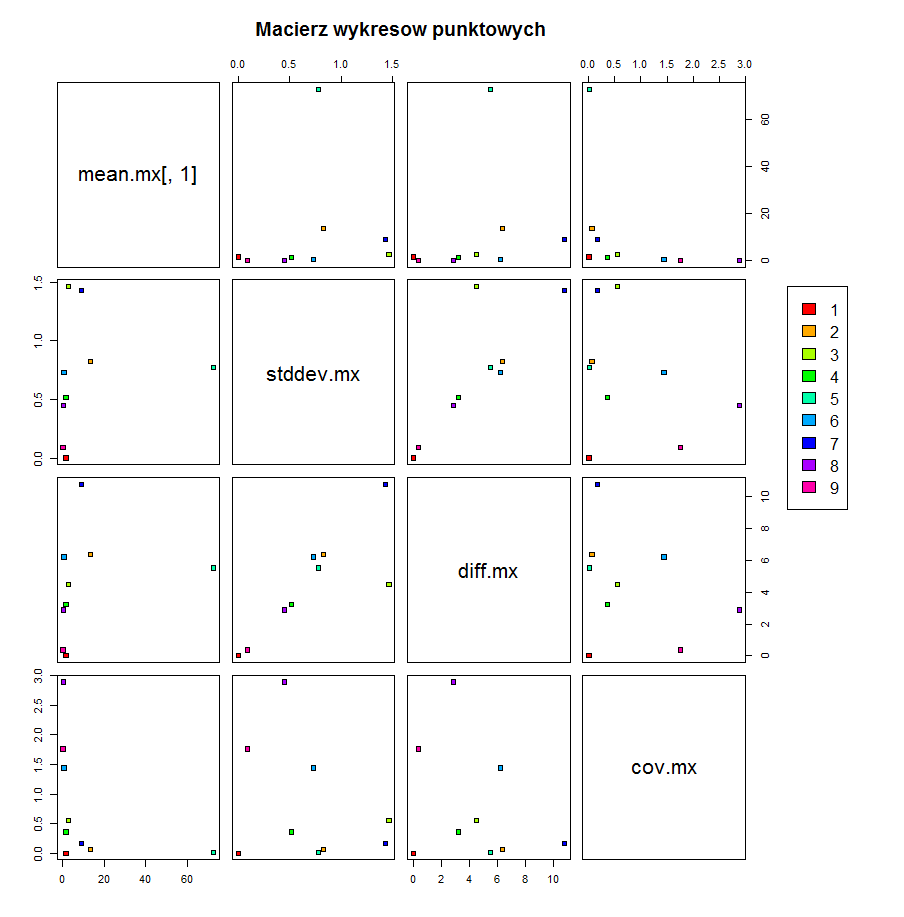
\includegraphics[width=.90\textwidth]{img/3_macierz_wykresow_punktowych.png}
\end{center}

Analizując powyższy schemat zauważamy pewne grupowania wśród atrybutów:

\begin{enumerate}
\item mean / stddev
  \begin{itemize}
  \item 1,9
  \item 2,4,6,8
  \item 3,7
  \item bez grupy: 5
  \end{itemize}
\item mean / diff
  \begin{itemize}
  \item 1,9
  \item 2,3,4,6,8
  \item bez grupy: 5,7
  \end{itemize}
\item mean / cov
  \begin{itemize}
  \item 1,2,3,4,7
  \item 6,9
  \item bez grupy: 5,8
  \end{itemize}
\item stddev / diff
  \begin{itemize}
  \item 1,9
  \item 4,8
  \item 2,5,6
  \item bez grupy: 3,7
  \end{itemize}
\item stddev / cov
  \begin{itemize}
  \item 2,4,5
  \item 3,7
  \item bez grupy: 1,6,8,9
  \end{itemize}
\item diff / cov
  \begin{itemize}
  \item 2,3,4,5
  \item bez grupy: 1,6,7,8,9
  \end{itemize}
\end{enumerate}
\medskip

\noindent
Skróty:
\begin{itemize}
\item \texttt{1,2,3...} - numery odpowiadających im atrybutów
\item \texttt{mean.mx[,1]} - średnia arytmetyczna
\item \texttt{stddev.m}x - odchylenie standardowe
\item \texttt{diff.mx} - rozstęp
\item \texttt{cov.mx} - miara zmienności
\end{itemize}

%%%%%%%%%%%%%%%%%%%%%%%%%%%%%%%%%%%%%%%%%%%%%%%%%%%%%%%%%%%%%%%%
\section{Zadanie 4}
\bigskip
%%%%%%%%%%%%%%%%%%%%%%%%%%%%%%%%%%%%%%%%%%%%%%%%%%%%%%%%%%%%%%%%

W związku z faktem, że nasze dane nie są współmierne, gdyż zakresy zmiennosci atrybutów znacznie
się różnią (patrz ``Zadanie 1''), warto poddać je przekształceniom, które pozwoliłyby nam lepiej
je porównać.

Wykresy z Zadania 2 pokazują, że w danych występuje dużo punktów oddalonych (pomijając atrybut nr.3).
Logicznym posunięciem będzie więc modyfikacja danych za pomocą procesu \textbf{standaryzacji} - metodą
znacznie mniej podatną na owe punkty oddalone.

Tym sposobem znacznie lepiej określimy bliskość poszczególnych wartości do wartości średniej.
Po standaryzacji otrzymujemy zakres zmiennosci \texttt{[-1, 1]}., gdzie znak określa czy dana jest
mniejsza/wieksza od średniej, a liczba o ile.

\medskip
\begin{lstlisting}
  # Standaryzacja
  data.std.mx <- matrix( , nrow = data.row, ncol = data.col)

  for(i in 1 : data.row) {
    for(j in 1 : data.col) {
      data.std.mx[i,j] <- (data.mx[i,j] - mean.mx[j,1]) / stddev.mx[j,1]
    }
  }

  # Graficzne przedstawienie danych std. za pomoca wykresu pudelkowego
  dev.new()
  boxplot(data.std.mx,
          xlab = "Atrybut",
          ylab = "Std. wartosc",
          main = "Graficzne przedstawienie wartosci po standaryzacji")
  }
\end{lstlisting}

\begin{center}
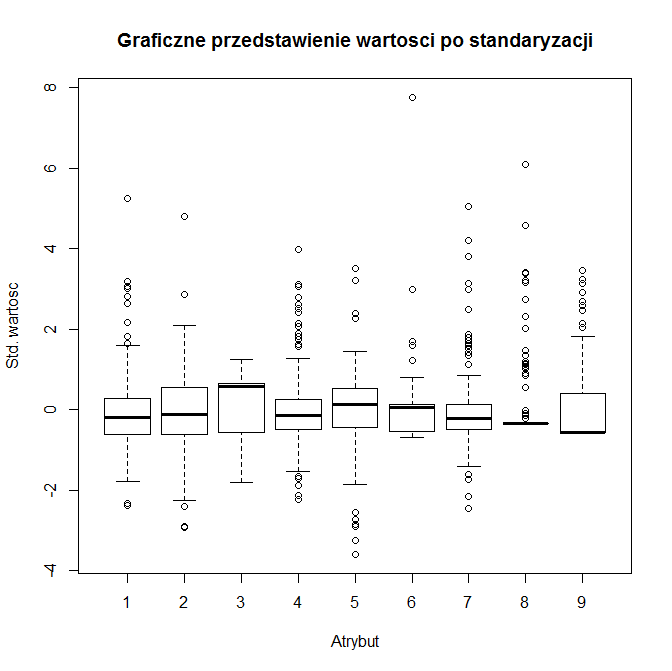
\includegraphics[width=.90\textwidth]{img/4_standaryzacja.png}
\end{center}

Na wykresie widzimy, że dane nie mieszczą się w zakresie \texttt{[-1, 1]}. Wpływają na to liczne punkty oddalone.
Jednak po procesie standaryzacji, mamy znacznie lepszą możliwość porównania danych.

%%%%%%%%%%%%%%%%%%%%%%%%%%%%%%%%%%%%%%%%%%%%%%%%%%%%%%%%%%%%%%%%%%%%%%%%%%%%%%%%%%%%%%%%%%%%%%%%%%%%%
\section{Podsumowanie}
\bigskip
%%%%%%%%%%%%%%%%%%%%%%%%%%%%%%%%%%%%%%%%%%%%%%%%%%%%%%%%%%%%%%%%%%%%%%%%%%%%%%%%%%%%%%%%%%%%%%%%%%%%


%%%%%%%%%%%%%%%%%%%%%%%%%%%%%%%%%%%%%%%%%%%%%%%%%%%%%%%%%%%%%
\end{document}
